\section{Implementation}

% 1) definition of the problems tackled
% 1.1) Girvan-Newman: description, goal, motivation, guidelines
% 1.2) Function renaming: description, goal, motivation, guidelines

% 2) Girvan-Newman approximation

% data gathering process

% Experiments list (main task and side analysis)


% 3) Function renaming

% data gathering process
% labelling discussion

% Experiments list (each attempt with different datasets, baselines, nlp and ggnn)




\begin{figure}[H]
    \centering
        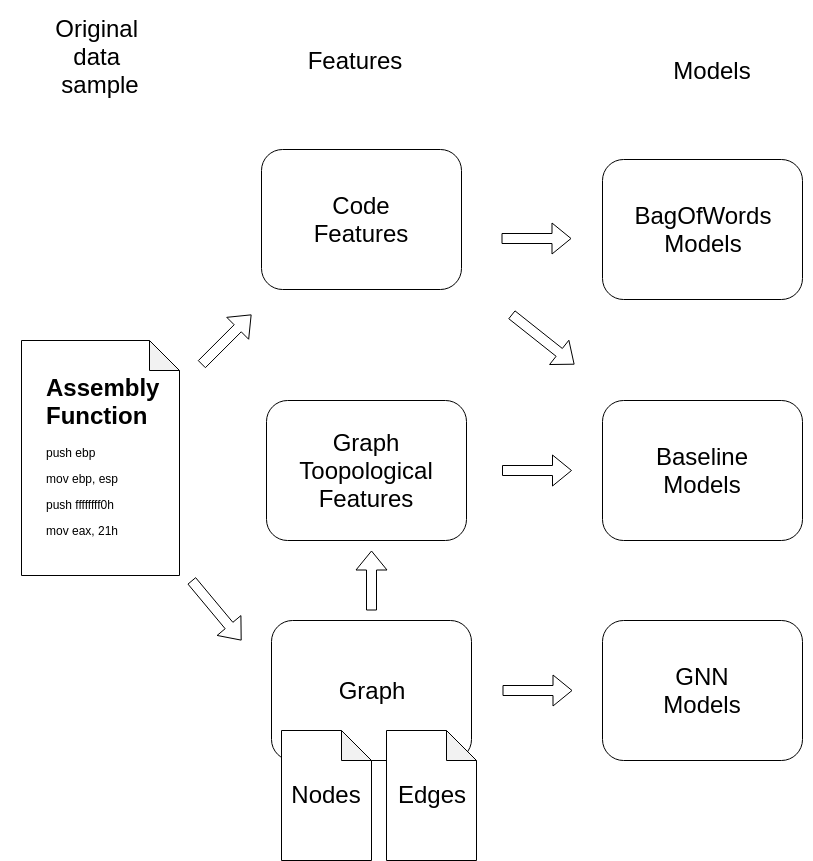
\includegraphics[width=0.95\linewidth]{img/Features_and_models_diagram.png}
    \caption{Features exracted from the dataset samples and their relationship with the models trained}\label{fig:Features_diagram}
\end{figure}



Building the dataset:
	- for girvan-newmann use well known datastsets available from PyG
	- not any available dataset, -> selection of binaries + compilation with symbols 
	 + manual labelling
	labelling problem, choosing the correct granularity of the label (each binary a label= a lot of noise since all binaries have almost all functionalities implemented, topics=10 classes, topics-task but summarized=24 classes, fine grained topic-task=170 clases)
